% Options for packages loaded elsewhere
% Options for packages loaded elsewhere
\PassOptionsToPackage{unicode}{hyperref}
\PassOptionsToPackage{hyphens}{url}
\PassOptionsToPackage{dvipsnames,svgnames,x11names}{xcolor}
%
\documentclass[
  authoryear,
  preprint]{elsarticle}
\usepackage{xcolor}
\usepackage{amsmath,amssymb}
\setcounter{secnumdepth}{5}
\usepackage{iftex}
\ifPDFTeX
  \usepackage[T1]{fontenc}
  \usepackage[utf8]{inputenc}
  \usepackage{textcomp} % provide euro and other symbols
\else % if luatex or xetex
  \usepackage{unicode-math} % this also loads fontspec
  \defaultfontfeatures{Scale=MatchLowercase}
  \defaultfontfeatures[\rmfamily]{Ligatures=TeX,Scale=1}
\fi
\usepackage{lmodern}
\ifPDFTeX\else
  % xetex/luatex font selection
\fi
% Use upquote if available, for straight quotes in verbatim environments
\IfFileExists{upquote.sty}{\usepackage{upquote}}{}
\IfFileExists{microtype.sty}{% use microtype if available
  \usepackage[]{microtype}
  \UseMicrotypeSet[protrusion]{basicmath} % disable protrusion for tt fonts
}{}
\makeatletter
\@ifundefined{KOMAClassName}{% if non-KOMA class
  \IfFileExists{parskip.sty}{%
    \usepackage{parskip}
  }{% else
    \setlength{\parindent}{0pt}
    \setlength{\parskip}{6pt plus 2pt minus 1pt}}
}{% if KOMA class
  \KOMAoptions{parskip=half}}
\makeatother
% Make \paragraph and \subparagraph free-standing
\makeatletter
\ifx\paragraph\undefined\else
  \let\oldparagraph\paragraph
  \renewcommand{\paragraph}{
    \@ifstar
      \xxxParagraphStar
      \xxxParagraphNoStar
  }
  \newcommand{\xxxParagraphStar}[1]{\oldparagraph*{#1}\mbox{}}
  \newcommand{\xxxParagraphNoStar}[1]{\oldparagraph{#1}\mbox{}}
\fi
\ifx\subparagraph\undefined\else
  \let\oldsubparagraph\subparagraph
  \renewcommand{\subparagraph}{
    \@ifstar
      \xxxSubParagraphStar
      \xxxSubParagraphNoStar
  }
  \newcommand{\xxxSubParagraphStar}[1]{\oldsubparagraph*{#1}\mbox{}}
  \newcommand{\xxxSubParagraphNoStar}[1]{\oldsubparagraph{#1}\mbox{}}
\fi
\makeatother

\usepackage{color}
\usepackage{fancyvrb}
\newcommand{\VerbBar}{|}
\newcommand{\VERB}{\Verb[commandchars=\\\{\}]}
\DefineVerbatimEnvironment{Highlighting}{Verbatim}{commandchars=\\\{\}}
% Add ',fontsize=\small' for more characters per line
\usepackage{framed}
\definecolor{shadecolor}{RGB}{241,243,245}
\newenvironment{Shaded}{\begin{snugshade}}{\end{snugshade}}
\newcommand{\AlertTok}[1]{\textcolor[rgb]{0.68,0.00,0.00}{#1}}
\newcommand{\AnnotationTok}[1]{\textcolor[rgb]{0.37,0.37,0.37}{#1}}
\newcommand{\AttributeTok}[1]{\textcolor[rgb]{0.40,0.45,0.13}{#1}}
\newcommand{\BaseNTok}[1]{\textcolor[rgb]{0.68,0.00,0.00}{#1}}
\newcommand{\BuiltInTok}[1]{\textcolor[rgb]{0.00,0.23,0.31}{#1}}
\newcommand{\CharTok}[1]{\textcolor[rgb]{0.13,0.47,0.30}{#1}}
\newcommand{\CommentTok}[1]{\textcolor[rgb]{0.37,0.37,0.37}{#1}}
\newcommand{\CommentVarTok}[1]{\textcolor[rgb]{0.37,0.37,0.37}{\textit{#1}}}
\newcommand{\ConstantTok}[1]{\textcolor[rgb]{0.56,0.35,0.01}{#1}}
\newcommand{\ControlFlowTok}[1]{\textcolor[rgb]{0.00,0.23,0.31}{\textbf{#1}}}
\newcommand{\DataTypeTok}[1]{\textcolor[rgb]{0.68,0.00,0.00}{#1}}
\newcommand{\DecValTok}[1]{\textcolor[rgb]{0.68,0.00,0.00}{#1}}
\newcommand{\DocumentationTok}[1]{\textcolor[rgb]{0.37,0.37,0.37}{\textit{#1}}}
\newcommand{\ErrorTok}[1]{\textcolor[rgb]{0.68,0.00,0.00}{#1}}
\newcommand{\ExtensionTok}[1]{\textcolor[rgb]{0.00,0.23,0.31}{#1}}
\newcommand{\FloatTok}[1]{\textcolor[rgb]{0.68,0.00,0.00}{#1}}
\newcommand{\FunctionTok}[1]{\textcolor[rgb]{0.28,0.35,0.67}{#1}}
\newcommand{\ImportTok}[1]{\textcolor[rgb]{0.00,0.46,0.62}{#1}}
\newcommand{\InformationTok}[1]{\textcolor[rgb]{0.37,0.37,0.37}{#1}}
\newcommand{\KeywordTok}[1]{\textcolor[rgb]{0.00,0.23,0.31}{\textbf{#1}}}
\newcommand{\NormalTok}[1]{\textcolor[rgb]{0.00,0.23,0.31}{#1}}
\newcommand{\OperatorTok}[1]{\textcolor[rgb]{0.37,0.37,0.37}{#1}}
\newcommand{\OtherTok}[1]{\textcolor[rgb]{0.00,0.23,0.31}{#1}}
\newcommand{\PreprocessorTok}[1]{\textcolor[rgb]{0.68,0.00,0.00}{#1}}
\newcommand{\RegionMarkerTok}[1]{\textcolor[rgb]{0.00,0.23,0.31}{#1}}
\newcommand{\SpecialCharTok}[1]{\textcolor[rgb]{0.37,0.37,0.37}{#1}}
\newcommand{\SpecialStringTok}[1]{\textcolor[rgb]{0.13,0.47,0.30}{#1}}
\newcommand{\StringTok}[1]{\textcolor[rgb]{0.13,0.47,0.30}{#1}}
\newcommand{\VariableTok}[1]{\textcolor[rgb]{0.07,0.07,0.07}{#1}}
\newcommand{\VerbatimStringTok}[1]{\textcolor[rgb]{0.13,0.47,0.30}{#1}}
\newcommand{\WarningTok}[1]{\textcolor[rgb]{0.37,0.37,0.37}{\textit{#1}}}

\usepackage{longtable,booktabs,array}
\usepackage{calc} % for calculating minipage widths
% Correct order of tables after \paragraph or \subparagraph
\usepackage{etoolbox}
\makeatletter
\patchcmd\longtable{\par}{\if@noskipsec\mbox{}\fi\par}{}{}
\makeatother
% Allow footnotes in longtable head/foot
\IfFileExists{footnotehyper.sty}{\usepackage{footnotehyper}}{\usepackage{footnote}}
\makesavenoteenv{longtable}
\usepackage{graphicx}
\makeatletter
\newsavebox\pandoc@box
\newcommand*\pandocbounded[1]{% scales image to fit in text height/width
  \sbox\pandoc@box{#1}%
  \Gscale@div\@tempa{\textheight}{\dimexpr\ht\pandoc@box+\dp\pandoc@box\relax}%
  \Gscale@div\@tempb{\linewidth}{\wd\pandoc@box}%
  \ifdim\@tempb\p@<\@tempa\p@\let\@tempa\@tempb\fi% select the smaller of both
  \ifdim\@tempa\p@<\p@\scalebox{\@tempa}{\usebox\pandoc@box}%
  \else\usebox{\pandoc@box}%
  \fi%
}
% Set default figure placement to htbp
\def\fps@figure{htbp}
\makeatother





\setlength{\emergencystretch}{3em} % prevent overfull lines

\providecommand{\tightlist}{%
  \setlength{\itemsep}{0pt}\setlength{\parskip}{0pt}}



 
\usepackage[]{natbib}
\bibliographystyle{elsarticle-harv}


\usepackage{booktabs}
\usepackage{caption}
\usepackage{longtable}
\usepackage{colortbl}
\usepackage{array}
\usepackage{anyfontsize}
\usepackage{multirow}
\makeatletter
\@ifpackageloaded{tcolorbox}{}{\usepackage[skins,breakable]{tcolorbox}}
\@ifpackageloaded{fontawesome5}{}{\usepackage{fontawesome5}}
\definecolor{quarto-callout-color}{HTML}{909090}
\definecolor{quarto-callout-note-color}{HTML}{0758E5}
\definecolor{quarto-callout-important-color}{HTML}{CC1914}
\definecolor{quarto-callout-warning-color}{HTML}{EB9113}
\definecolor{quarto-callout-tip-color}{HTML}{00A047}
\definecolor{quarto-callout-caution-color}{HTML}{FC5300}
\definecolor{quarto-callout-color-frame}{HTML}{acacac}
\definecolor{quarto-callout-note-color-frame}{HTML}{4582ec}
\definecolor{quarto-callout-important-color-frame}{HTML}{d9534f}
\definecolor{quarto-callout-warning-color-frame}{HTML}{f0ad4e}
\definecolor{quarto-callout-tip-color-frame}{HTML}{02b875}
\definecolor{quarto-callout-caution-color-frame}{HTML}{fd7e14}
\makeatother
\makeatletter
\@ifpackageloaded{caption}{}{\usepackage{caption}}
\AtBeginDocument{%
\ifdefined\contentsname
  \renewcommand*\contentsname{Table of contents}
\else
  \newcommand\contentsname{Table of contents}
\fi
\ifdefined\listfigurename
  \renewcommand*\listfigurename{List of Figures}
\else
  \newcommand\listfigurename{List of Figures}
\fi
\ifdefined\listtablename
  \renewcommand*\listtablename{List of Tables}
\else
  \newcommand\listtablename{List of Tables}
\fi
\ifdefined\figurename
  \renewcommand*\figurename{Figure}
\else
  \newcommand\figurename{Figure}
\fi
\ifdefined\tablename
  \renewcommand*\tablename{Table}
\else
  \newcommand\tablename{Table}
\fi
}
\@ifpackageloaded{float}{}{\usepackage{float}}
\floatstyle{ruled}
\@ifundefined{c@chapter}{\newfloat{codelisting}{h}{lop}}{\newfloat{codelisting}{h}{lop}[chapter]}
\floatname{codelisting}{Listing}
\newcommand*\listoflistings{\listof{codelisting}{List of Listings}}
\makeatother
\makeatletter
\makeatother
\makeatletter
\@ifpackageloaded{caption}{}{\usepackage{caption}}
\@ifpackageloaded{subcaption}{}{\usepackage{subcaption}}
\makeatother
\journal{Journal Name}
\usepackage{bookmark}
\IfFileExists{xurl.sty}{\usepackage{xurl}}{} % add URL line breaks if available
\urlstyle{same}
\hypersetup{
  pdftitle={Responsive Robotics to Increase Trust in Autonomous Human--Robot Interaction},
  pdfauthor={M.C. Lau; Shauna Heron},
  pdfkeywords={human-robot interaction, HRI, socially assistive
robotics, cobots, autonomous robot systems, spoken language
interaction, trust in automation, trust in human-robot
interaction, affect-adaptive systems},
  colorlinks=true,
  linkcolor={blue},
  filecolor={Maroon},
  citecolor={Blue},
  urlcolor={Blue},
  pdfcreator={LaTeX via pandoc}}


\setlength{\parindent}{6pt}
\begin{document}

\begin{frontmatter}
\title{Responsive Robotics to Increase Trust in Autonomous Human--Robot
Interaction \\\large{An In-Person Pilot Study} }
\author[1]{M.C. Lau%
\corref{cor1}%
\fnref{fn1}}
 \ead{mclau@laurentian.ca} 
\author[1]{Shauna Heron%
%
\fnref{fn2}}
 \ead{sheron@laurentian.ca} 

\affiliation[1]{organization={Laurentian University, Bharti School of
Engineering},,postcodesep={}}
\affiliation[2]{organization={Laurentian University, School of Social
Sciences},,postcodesep={}}

\cortext[cor1]{Corresponding author}
\fntext[fn1]{This is the first author footnote.}
\fntext[fn2]{Another author footnote, this is a very long footnote and
it should be a really long footnote. But this footnote is not yet
sufficiently long enough to make two lines of footnote text.}
        
\begin{abstract}
This study implements a multi-stage collaborative task system where
participants collaborate with the Misty-II social robot to solve a
who-dunnit type task. The system utilizes an autonomous,
mixed-initiative dialogue architecture with affect-responsive
capabilities.
\end{abstract}





\begin{keyword}
    human-robot interaction \sep HRI \sep socially assistive
robotics \sep cobots \sep autonomous robot systems \sep spoken language
interaction \sep trust in automation \sep trust in human-robot
interaction \sep 
    affect-adaptive systems
\end{keyword}
\end{frontmatter}
    

\subsection{Introduction}\label{introduction}

As automation expands across safety-critical domains such as
manufacturing, healthcare, and mining, robotic systems are increasingly
expected to operate alongside humans rather than in isolation
\citep{fu2021, racette2024}. In these collaborative settings, successful
deployment depends not only on technical performance but on whether
human users are willing to rely on, communicate with, and coordinate
their actions around autonomous systems
\citep{campagna2025, emaminejad2022}. Trust has therefore emerged as a
central determinant of adoption and effective use in human--robot
collaboration (HRC). Insufficient trust can lead to disuse or rejection
of automation, whereas excessive trust risks overreliance and automation
bias, particularly in environments characterized by uncertainty or
incomplete information \citep{devisser2020}.

A substantial body of human--robot interaction (HRI) research has
examined how robot behavior shapes user trust, perceived reliability,
and cooperation \citep{shayganfar2019, fartook2025}. Prior work has
demonstrated that trust influences both subjective evaluations of
robotic partners and objective outcomes such as compliance, task
performance, and collaborative efficiency. However, much of this
literature relies on interactions conducted under highly controlled
conditions, including scripted behaviors, simulated environments, or
Wizard-of-Oz paradigms in which a human operator covertly manages
aspects of the robot's behavior. While these approaches are valuable for
isolating specific design factors, they often obscure the interaction
breakdowns and system imperfections that characterize real-world
autonomous robots.

In deployed systems, limitations such as speech recognition errors,
delayed responses, misinterpretations of user intent, and incomplete
affect sensing are not peripheral issues but defining features of
interaction. These failures are likely to play a decisive role in
shaping trust and collaboration, yet remain underrepresented in
empirical HRI research. Understanding how trust emerges---and sometimes
deteriorates---under realistic autonomous conditions is therefore
critical for the design of robots intended for real-world collaborative
use.

One proposed mechanism for supporting trust in HRI is
\textbf{responsiveness}: the extent to which a robot adapts its behavior
based on user state and interaction context
\citep{shayganfar2019, fartook2025}. Responsive robots may adjust their
dialogue, timing, or support strategies in response to inferred
affective cues such as confusion, frustration, or disengagement. Prior
studies suggest that such adaptive behavior can enhance perceived social
intelligence and trustworthiness, particularly in dialogue-driven tasks
\citep{birnbaum2016}. However, most evidence for these effects comes
from simulated or semi-autonomous systems, leaving open questions about
how responsiveness operates when implemented in fully autonomous,
in-person interactions.

From an engineering perspective, responsiveness represents an
interaction policy rather than a superficial social cue. Proactive,
state-contingent assistance differs fundamentally from reactive,
request-based behavior, particularly when implemented under strict
autonomy constraints. Designing and evaluating such policies requires
systems capable of managing spoken-language dialogue, maintaining
interaction state, and coordinating verbal and nonverbal responses in
real time---while remaining robust to noise, latency, and sensing
errors.

The present work addresses these gaps through a pilot study examining
trust and collaboration during in-person interaction with a fully
autonomous social robot. Participants collaborated with one of two
versions of the same robot platform during a dialogue-driven puzzle task
requiring shared problem solving. In both conditions, all interaction
management---including speech recognition, dialogue state tracking, task
progression, and response generation---was handled autonomously by the
robot without human intervention. In the \textbf{responsive} condition,
the robot employed a proactive interaction policy, adapting its
assistance based on conversational cues and inferred user affect. In the
\textbf{neutral} condition, the robot followed a reactive policy,
providing assistance only when explicitly requested.

This study was conducted as a pilot with three primary objectives: (1)
to evaluate the feasibility of deploying an autonomous spoken-language
interaction system with affect-responsive behavior on a mobile robot
platform; (2) to assess whether differences in interaction policy
influence trust, perceived social intelligence, and collaborative
experience under realistic autonomous conditions; and (3) to examine how
individual differences in baseline attitudes toward robots and cognitive
engagement may moderate responses to adaptive robotic behavior. Rather
than optimizing for flawless interaction, the system was intentionally
designed to reflect the capabilities and limitations of contemporary
social robots, allowing interaction breakdowns to surface naturally.

An additional objective of this pilot study was to inform the design of
an autonomous affect-adaptive interaction system under real-time
constraints. The initial system concept included multimodal affect
inference based on facial expressions, vocal prosody, and interaction
dynamics. However, early integration testing revealed substantial
challenges related to latency, model orchestration, and timing
sensitivity when deploying multiple perception models concurrently on an
edge-supported mobile robot platform. Given the small-scale nature of
the pilot and the central importance of maintaining stable, real-time
dialogue, the deployed system prioritized robustness of spoken-language
interaction and dialogue-based affect inference over broader multimodal
sensing. Affect adaptation in this study was therefore driven primarily
by speech-based affect signals and conversational context, allowing us
to evaluate responsiveness within a fully autonomous interaction while
preserving realistic system constraints.

By combining post-interaction trust measures with task-level and
behavioral observations, this pilot study aims to contribute empirical
evidence on how trust in human--robot collaboration emerges in fully
autonomous settings. The findings are intended to inform the design of a
larger, subsequent study by identifying technical, interactional, and
methodological challenges---including speech recognition limitations,
language barriers, and interaction design trade-offs---that must be
addressed when evaluating affect-responsive robots in real-world
contexts.

The remainder of this paper is structured as follows. Section 2 reviews
related work on spoken-language interaction, trust, and responsiveness
in HRI. Section 3 describes the autonomous system architecture,
experimental design, and measurement approach. Section 4 presents
results from the pilot study, followed by a discussion of implications,
limitations, and directions for future work.

\section{Methods}\label{methods}

\subsection{Experimental Design and
Conditions}\label{experimental-design-and-conditions}

This study employed a between-subjects experimental design to examine
how robot interaction policy influences trust and collaboration during
fully autonomous, in-person human--robot interaction. The sole
experimental factor was the robot's interaction policy, with
participants randomly assigned to interact with either a
\textbf{responsive} or \textbf{neutral} version of the same robot
system.

Participants interacted with a Misty-II social robot in a shared
physical workspace that included a participant-facing computer interface
\citep{mistya}. The interface was used to display task materials,
collect participant inputs, and manage task progression. Importantly,
the interface did not function as a control mechanism for the robot.
Instead, the robot autonomously monitored task state and participant
inputs via the interface and managed dialogue and behavior accordingly,
without real-time human intervention.

Random assignment to condition was performed at sign-up using Qualtrics.
Due to no-shows, last-minute cancellations, and technical exclusions
(described below), final group sizes were \emph{n} = 14 in the
RESPONSIVE condition and \emph{n} = 9 in the CONTROL condition.

\subsubsection{Interaction Policies}\label{interaction-policies}

\begin{itemize}
\item
  \textbf{RESPONSIVE condition (experimental):}\\
  The robot employed a proactive, affect-adaptive interaction policy.
  Robot responses were modulated based on inferred participant affect,
  dialogue context, and task demands, resulting in unsolicited
  encouragement, clarification, and engagement-oriented behaviors when
  appropriate.
\item
  \textbf{CONTROL condition (baseline):}\\
  The robot employed a neutral, reactive interaction policy. Assistance
  and information were provided only when explicitly requested by the
  participant, without affect-based adaptation or proactive support.
\end{itemize}

Both conditions used identical hardware, software infrastructure,
sensing capabilities, and task logic. The only difference between
conditions was the robot's interaction policy.

\subsubsection{Collaborative Task
Design}\label{collaborative-task-design}

Participants completed an immersive, narrative-driven puzzle game
consisting of five sequential stages and two timed reasoning tasks. The
game context positioned participants as investigators searching for a
missing robot colleague, with the robot serving as a diegetic guide and
collaborative partner. The overall interaction lasted approximately 15
minutes.

\begin{figure}

\centering{

\includegraphics[width=5.02083in,height=\textheight,keepaspectratio]{images/misty-pullback.jpg}

}

\caption{\label{fig-setup}Experimental setup showing the autonomous
robot and participant-facing task interface used during in-person
sessions. Participants entered task responses and navigated between task
stages using the interface, while the robot autonomously tracked task
state and adapted its interaction based on participant input. No
real-time human intervention occurred during the interaction.}

\end{figure}%

The task structure was designed to elicit collaboration under two
distinct dependency conditions: (1) enforced collaboration, where the
robot was required to complete the task, and (2) optional collaboration,
where participants could choose whether to engage the robot.

\paragraph{Stage Overview}\label{stage-overview}

\begin{enumerate}
\def\labelenumi{\arabic{enumi}.}
\tightlist
\item
  \textbf{Greeting:} The robot introduced itself and engaged in brief
  rapport-building dialogue.\\
\item
  \textbf{Mission Brief:} The robot explained the narrative context and
  overall objectives.\\
\item
  \textbf{Task 1:} Robot-dependent collaborative reasoning task.\\
\item
  \textbf{Task 2:} Open-ended problem solving with optional robot
  support.\\
\item
  \textbf{Wrap-up:} The robot provided closing feedback and concluded
  the interaction.
\end{enumerate}

Participants advanced between stages using the interface, either at the
robot's prompting or at their own discretion. All spoken dialogue and
interaction events were logged automatically.

\paragraph{Task 1: Robot-Dependent Collaborative
Reasoning}\label{task-1-robot-dependent-collaborative-reasoning}

In Task 1, participants were required to identify a suspect from a 6 × 4
grid of 24 candidates by asking the robot a series of yes/no questions
about the suspect's features (e.g., clothing, accessories). The grid was
displayed on the interface, while questions were posed verbally.

\begin{figure}

\centering{

\includegraphics[width=5.02083in,height=\textheight,keepaspectratio]{images/task1-whodunnit.png}

}

\caption{\label{fig-task1}In the first task, participants were required
to identify a suspect from a 6 × 4 grid of 24 candidates by asking the
robot a series of yes/no questions about the suspect's features (e.g.,
hair color, accessories, clothing). The grid was displayed on the
interface, while questions were posed verbally to the robot.
Participants could track those eliminated here and input their final
answer.}

\end{figure}%

The robot possessed ground-truth information necessary to answer each
question correctly. Successful task completion was therefore dependent
on interaction with the robot, creating a forced collaborative dynamic.
Participants were required to coordinate questioning strategies with the
robot to narrow down the suspect within a five-minute time limit. The
structured nature of the task ensured consistent interaction demands
across participants and conditions.

\paragraph{Task 2: Open-Ended Collaborative Problem
Solving}\label{task-2-open-ended-collaborative-problem-solving}

Task 2 involved a more open-ended reasoning challenge. Participants were
presented with multiple technical logs through a simulated terminal
interface that could be used to infer the location of the missing robot.

\begin{figure}

\centering{

\includegraphics[width=5.02083in,height=\textheight,keepaspectratio]{images/task2-cryptic-puzzle.png}

}

\caption{\label{fig-task2}The task 2 interface presented multiple
technical logs through a simulated terminal interface that could be used
to determine the location of the missing robot.}

\end{figure}%

Unlike Task 1, the robot did not have access to ground-truth information
or the contents of the logs. The robot's assistance was limited to
general reasoning support derived from its language model, such as
explaining how to interpret log formats, suggesting problem-solving
strategies, or prompting participants to reflect on inconsistencies.

Participants could complete this task independently or solicit
assistance from the robot at their discretion \citep{lin2022}. This
design allowed collaboration to emerge voluntarily rather than being
enforced by task structure, positioning the robot as an advisory partner
rather than an authoritative source.

\subsubsection{Study Protocol}\label{study-protocol}

In-person sessions were conducted in a quiet, private room at Laurentian
University between November and December. Prior to each session, the
robot's interaction policy was configured to the assigned experimental
condition.

Upon arrival, participants were greeted by the researcher, provided with
a brief overview of the session, and given instructions for effective
communication with the robot, including waiting for a visual indicator
before speaking. Once participants indicated readiness, the researcher
exited the room, leaving the participant and robot to complete the
interaction without human presence or observation. Participants
initiated the interaction by clicking a start button on the interface
and were informed that they could terminate the session at any time
without penalty.

Following task completion, participants completed a post-interaction
questionnaire assessing trust. Participants then engaged in a brief
debrief with the researcher. Total session duration averaged
approximately 30 minutes.

\subsubsection{Measures}\label{measures}

A combination of self-report and objective measures was used to assess
trust, engagement, and task performance.

\paragraph{Self-Report Measures}\label{self-report-measures}

Participants completed a pre-session questionnaire assessing baseline
characteristics, including the Negative Attitudes Toward Robots Scale
(NARS) and the short form of the Need for Cognition scale (NFC-s). These
measures were used to capture individual differences that may moderate
responses to robot interaction.

Post-interaction trust was assessed using two validated instruments: the
Trust Perception Scale--HRI and the Trust in Industrial Human--Robot
Collaboration scale \citep{bartneck2009, charalambous}. Together, these
measures capture multiple dimensions of trust, including perceived
reliability, competence, and collaborative suitability.

\paragraph{Objective and Behavioral
Measures}\label{objective-and-behavioral-measures}

Objective task metrics included task completion, task accuracy, time to
completion, and the number of assistance requests made to the robot.
Behavioral engagement metrics were derived from interaction logs and
manually coded dialogue transcripts, including number of dialogue turns,
frequency of communication breakdowns, response timing, and
task-relevant robot contributions.

\subsubsection{Participants, Communication Viability, and Analytic
Strategy}\label{participants-communication-viability-and-analytic-strategy}

A total of 29 participants were recruited from the Laurentian University
community via word of mouth and the SONA recruitment system. Eligibility
criteria included being 18 years or older, fluent in spoken and written
English, and having normal or corrected-to-normal hearing and vision.
Participants received a \$15 gift card as compensation for their time.
All procedures were approved by the Laurentian University Research
Ethics Board (REB \#6021966).

Although English fluency was an eligibility requirement, post-hoc review
of interaction transcripts and system logs revealed that a subset of
sessions exhibited severe and sustained communication failure. In these
sessions, automatic speech recognition (ASR) output was largely
unintelligible or fragmented, preventing the robot from extracting
sufficient linguistic content to maintain dialogue, respond meaningfully
to participant queries, or support task progression. As a result,
interaction frequently stalled, participant questions went unanswered or
were misinterpreted, and collaborative problem-solving was effectively
impossible. These sessions did not reflect degraded interaction quality
but rather a complete breakdown of language-mediated communication,
rendering the experimental manipulation inoperative.

Because the study relied fundamentally on spoken-language collaboration,
sessions exhibiting persistent communication failure were classified as
\textbf{protocol non-adherence} and excluded from task-level analyses
(\emph{n} = 6). Exclusion decisions were based solely on communication
viability and interaction mechanics, not on task outcomes or trust
measures.

To ensure transparency and to evaluate the impact of communication-based
exclusions, analyses were conducted in three stages. First, the
\textbf{eligible-sample analysis} (excluding non-viable sessions) was
treated as the primary analysis because it reflects interactions in
which the spoken-language protocol---and therefore the experimental
manipulation---operated as intended. Second, a \textbf{full-sample
analysis} including all participants was conducted as a sensitivity test
to evaluate robustness to communication failures and protocol
deviations. Third, a \textbf{mechanism-focused analysis} compared
excluded and included sessions on interaction-process metrics (e.g., ASR
failure rates, dialogue turn completion, task abandonment) to quantify
how severe communication breakdown alters the interaction dynamics and
renders the manipulation inoperative.

It is important to note that while full-sample analyses are informative
as robustness checks, trust measures obtained from sessions with
complete communication breakdown are not interpreted as valid estimates
of human--robot trust in the intended sense. In these cases, the robot
was unable to sustain dialogue or collaborative behavior, meaning that
participants could not meaningfully evaluate reliability, competence, or
collaborative intent. Full-sample analyses are therefore treated as
sensitivity analyses reflecting real-world failure conditions, rather
than as alternative estimates of trust under functional interaction.

Across analyses, participants in the responsive and control conditions
were comparable with respect to demographic characteristics, prior
experience with robots, and baseline attitudes toward robots, including
Negative Attitudes Toward Robots (NARS) and Need for Cognition scores
\citep{nomura2006, cacioppo1984, cacioppo1996}.

\section{Results}\label{results}

\subsection{Communication Viability and Analytic
Samples}\label{communication-viability-and-analytic-samples}

Prior to hypothesis testing, interaction sessions were classified based
on communication viability using a dialogue-level metric derived from
system logs and manual coding. Specifically, the proportion of dialogue
turns affected by speech-recognition failure or fragmented utterances
was computed for each session. Sessions in which more than 60\% of
dialogue turns were characterized by communication breakdown were
classified as non-viable (n=6). This criterion closely matched sessions
independently flagged during administration and reflects cases in which
sustained spoken-language interaction was not possible.

Of the 29 completed sessions, 6 were classified as non-viable due to
severe and persistent communication failure (i.e., unintelligble
sentence fragments). Because the experimental manipulation relied on
language-mediated collaboration, analyses were conducted using three
complementary approaches: (1) a primary \textbf{eligible-sample
analysis} excluding non-viable sessions, (2) a \textbf{full-sample
sensitivity analysis} including all sessions, and (3) a
\textbf{mechanism-focused analysis} examining how communication
breakdown altered interaction dynamics.

Unless otherwise noted, inferential results reported below refer to the
eligible sample.

\subsection{Primary Analysis: Eligible
Sample}\label{primary-analysis-eligible-sample}

\subsubsection{Descriptive Outcomes}\label{descriptive-outcomes}

\begin{table}
\fontsize{10.0pt}{12.0pt}\selectfont
\begin{tabular*}{\linewidth}{@{\extracolsep{\fill}}lcccc}
\toprule
\textbf{Characteristic} & \textbf{N} & \textbf{CONTROL}  N = 9\textsuperscript{\textit{1}} & \textbf{RESPONSIVE}  N = 14\textsuperscript{\textit{1}} & \textbf{p-value}\textsuperscript{\textit{2}} \\ 
\midrule\addlinespace[2.5pt]
Trust in Industrial HRI Collaboration & 23 & 41 (22) & 67 (21) & {\bfseries 0.007} \\ 
Subscales &  &  &  &  \\ 
    Reliability subscale & 23 & 41 (25) & 65 (18) & {\bfseries 0.022} \\ 
    Trust Perception subscale & 23 & 46 (21) & 60 (22) & 0.14 \\ 
    Affective Trust subscale & 23 & 52 (32) & 79 (22) & {\bfseries 0.030} \\ 
Trust Perception Scale\textendashHRI & 23 & 62 (15) & 77 (18) & {\bfseries 0.046} \\ 
Overall Task Accuracy & 23 & 0.60 (0.22) & 0.66 (0.23) & 0.49 \\ 
Dialogue Turns & 23 & 36 (7) & 33 (5) & 0.21 \\ 
Avg Task Duration (mins) & 23 & 13.82 (2.60) & 15.26 (2.12) & 0.16 \\ 
Avg Response Time (ms) & 23 & 13.21 (0.84) & 17.24 (2.52) & {\bfseries <0.001} \\ 
Silent Periods & 23 & 5.67 (2.06) & 4.71 (2.05) & 0.29 \\ 
Engaged Responses & 23 & 2.22 (2.22) & 3.50 (1.95) & 0.077 \\ 
Frustrated Responses & 23 & 0.56 (0.73) & 0.93 (1.21) & 0.58 \\ 
\bottomrule
\end{tabular*}
\begin{minipage}{\linewidth}
\textsuperscript{\textit{1}}Mean (SD)\\
\textsuperscript{\textit{2}}Wilcoxon rank sum test; Wilcoxon rank sum exact test\\
\end{minipage}
\end{table}

Descriptive comparisons of post-interaction trust measures indicated
higher trust ratings in the RESPONSIVE condition relative to the CONTROL
condition across both trust scales (Table X). Mean post-interaction
scores on the Trust Perception Scale--HRI were approximately
\emph{{[}insert value{]}} points higher in the responsive condition,
while scores on the Trust in Industrial Human--Robot Collaboration scale
differed by approximately \emph{{[}insert value{]}} points. Behavioral
summaries further indicated differences in dialogue patterns and robot
assistance behaviors consistent with the intended interaction policies.

Objective task accuracy did not differ between conditions across any
task-level measures except suspect accuracy (robot dependendant task),
indicating that increased trust was only attributable to improved task
success when interaction was necessary to complete accurately. This
suggests that observed differences in trust were not driven by
differential task success.

Despite similar task accuracy, interactions in the responsive condition
were characterized by longer durations, slower response times, and a
higher number of AI-detected engaged responses. These findings suggest
that responsiveness altered the interaction dynamics and affective tone
rather than task outcomes.

\subsubsection{Bayesian Hierarchical Models of Post-Interaction
Trust}\label{bayesian-hierarchical-models-of-post-interaction-trust}

To formally evaluate condition effects on post-interaction trust,
Bayesian hierarchical models were fitted separately for each trust
outcome. Models predicted post-interaction trust as a function of
interaction policy (RESPONSIVE vs.~CONTROL), with random intercepts for
session and trust scale items to account for repeated measurement and
item-level variability.

Across both trust measures, posterior estimates favored higher trust
ratings in the RESPONSIVE condition. For the Trust in Industrial
Human--Robot Collaboration scale, the estimated group difference was
\emph{{[}insert median{]}} points (95\% credible interval
{[}\emph{lower}, \emph{upper}{]}), with a posterior probability greater
than \emph{{[}insert{]}\%} that the effect exceeded a practically
meaningful threshold of five points on the 0--100 scale. Posterior mass
exceeding ten points was \emph{{[}insert{]}\%}, indicating a substantial
likelihood of a large effect.

For the Trust Perception Scale--HRI, the estimated group difference was
smaller and more uncertain (\emph{{[}insert median{]}} points; 95\%
credible interval {[}\emph{lower}, \emph{upper}{]}). Although the
credible interval included zero, the posterior probability that the
responsive condition increased trust was greater than
\emph{{[}insert{]}\%}, suggesting a consistent directional effect with
greater individual variability.

Sensitivity analyses using wider priors yielded nearly identical
posterior estimates, indicating that results were not driven by prior
specification.

\subsubsection{Sensitivity Analysis: Full
Sample}\label{sensitivity-analysis-full-sample}

Including sessions classified as non-viable increased variability and
attenuated estimated effect sizes across trust measures. As expected,
posterior uncertainty increased relative to the eligible-sample
analysis. However, directional trends favoring the RESPONSIVE condition
remained evident across both trust outcomes.

These results indicate that while communication breakdown weakens the
interpretability of trust measures, the overall pattern of results is
not solely an artifact of exclusion decisions. Full-sample analyses are
therefore treated as robustness checks reflecting real-world interaction
variability rather than as alternative estimates of trust under
functional interaction conditions.

\subsubsection{Mechanism Analysis: Communication Breakdown as a Failure
Mode}\label{mechanism-analysis-communication-breakdown-as-a-failure-mode}

To examine why communication-based exclusion was necessary, interaction
dynamics were compared between viable and non-viable sessions. Sessions
classified as non-viable were characterized by substantially higher
rates of speech-recognition failure, reduced dialogue coherence,
increased task abandonment, and limited task-relevant information
exchange.

Notably, under conditions of severe communication breakdown, the
RESPONSIVE robot continued to generate proactive assistance,
encouragement, and meta-communication aimed at repairing the
interaction. However, these efforts did not restore mutual understanding
and, in several cases, appeared to increase participant confusion and
cognitive load. In contrast, the CONTROL robot's reactive interaction
policy resulted in fewer unsolicited interventions, which---while less
supportive under normal conditions---reduced interaction complexity when
language-mediated collaboration was no longer viable.

As a result, trust ratings in non-viable sessions did not systematically
track the intended responsiveness manipulation. These findings suggest
that when spoken-language interaction collapses, higher-level constructs
such as trust and collaboration are no longer meaningfully instantiated.
Communication viability therefore represents a boundary condition for
evaluating affect-adaptive interaction policies in autonomous social
robots.

\subsection{Trust subscale patterns}\label{trust-subscale-patterns}

\subsection{Interaction dynamics and task
performance}\label{interaction-dynamics-and-task-performance}

\subsubsection{Task performance}\label{task-performance}

Objective task accuracy did not differ between conditions across any
task-level measures except suspect accuracy (robot dependendant task),
indicating that increased trust was only attributable to improved task
success when interaction was necessary to complete accurately.

Despite similar task accuracy, interactions in the responsive condition
were characterized by longer durations, slower response times, and a
higher number of AI-detected engaged responses. These findings suggest
that responsiveness altered the interaction dynamics and affective tone
rather than task outcomes.

\subsection{Individual differences and correlational
patterns}\label{individual-differences-and-correlational-patterns}

As expected, we found that higher Need for Cognition (NFC) scores were
negatively associated with Negative Attitudes Towards Robots (NARS),
indicating that individuals who enjoy effortful thinking tend to have
more positive attitudes towards robots. This relationship is consistent
with prior literature suggesting that cognitive engagement is associated
with openness to new technologies. In terms of NARS subscales, NFC was
negatively correlated with all three subscales, but significantly so
only in the domain of Situations of Interaction with Robots. This
suggests that individuals with higher NFC are less likely to hold
negative attitudes across various dimensions of robot interaction but
especially around direct interaction with robots.

--\textgreater{} how to talk about post-interaction correlations
w/pre-interaction measures Several behavioural and task-level measures
were correlated with post-interaction trust, consistent with the
interpretation that trust judgments were shaped by interaction quality;
these variables were not included as covariates in primary models to
avoid conditioning on potential mediators.

Baseline negative attitudes toward robots were negatively correlated
with post-interaction trust, with the strongest associations observed
for affective trust subscales. In contrast, objective task performance
was selectively associated with perceived reliability. Need for
cognition was negatively correlated with negative robot attitudes and
interaction-level negative affect, suggesting that individual
differences contributed to variability in trust responses.

\begin{figure}

\centering{

\pandocbounded{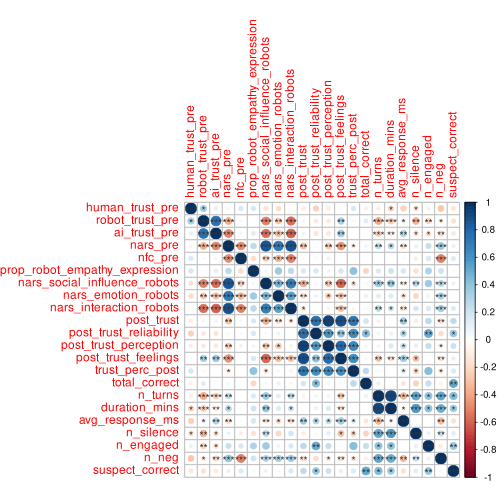
\includegraphics[keepaspectratio]{misty-paper_files/figure-pdf/fig-corr-1.pdf}}

}

\caption{\label{fig-corr}}

\end{figure}%

\subsubsection{Model robustness and predictive
checks}\label{model-robustness-and-predictive-checks}

Sensitivity analyses using alternative prior specifications yielded
substantively similar estimates, and leave-one-out cross-validation
indicated comparable predictive performance between models with and
without the group effect.

\begin{tcolorbox}[enhanced jigsaw, title=\textcolor{quarto-callout-important-color}{\faExclamation}\hspace{0.5em}{TO DO:}, colback=white, colframe=quarto-callout-important-color-frame, toptitle=1mm, titlerule=0mm, colbacktitle=quarto-callout-important-color!10!white, breakable, leftrule=.75mm, coltitle=black, rightrule=.15mm, opacityback=0, left=2mm, bottomtitle=1mm, arc=.35mm, toprule=.15mm, bottomrule=.15mm, opacitybacktitle=0.6]

\begin{itemize}
\tightlist
\item
  add subscale column to long format data
\item
  run an analysis of performance by robot-dependent versus
  robot-independent tasks
\item
  write up a future directions section for the planned larger study
\item
  talk about unexpected language issues with people signing up with
  difficultly speaking and understanding english which cuased problems
  with asr and interaction
\item
  run analysis of dialogue dynamics included Bertopic or some other
  analysis of the actual content of the conversations/interactions
\end{itemize}

\end{tcolorbox}

\begin{tcolorbox}[enhanced jigsaw, title=\textcolor{quarto-callout-important-color}{\faExclamation}\hspace{0.5em}{TODO2}, colback=white, colframe=quarto-callout-important-color-frame, toptitle=1mm, titlerule=0mm, colbacktitle=quarto-callout-important-color!10!white, breakable, leftrule=.75mm, coltitle=black, rightrule=.15mm, opacityback=0, left=2mm, bottomtitle=1mm, arc=.35mm, toprule=.15mm, bottomrule=.15mm, opacitybacktitle=0.6]

Manually score each dialogue series.

For each interaction and stage:

\begin{itemize}
\tightlist
\item
  did the participant ask for help?
\item
  how many times?
\item
  did the robot give useful help?
\item
  did the robot give misleading or incorrect help?
\item
  did the robot stick to the policy?
\item
  how many times did the robot fail to understand the participant?
\end{itemize}

For each task:

\begin{itemize}
\tightlist
\item
  is there evidence that the robot helped complete the task?
\item
  is there evidence that the participant solved the problem without
  help?
\end{itemize}

\end{tcolorbox}

\section{Discussion}\label{discussion}

Mention language confounders!! The present findings also highlight an
important boundary condition for trust measurement in spoken-language
HRI. When language-mediated interaction collapses entirely, higher-level
constructs such as trust and collaboration are no longer meaningfully
defined. Under such conditions, trust does not simply decrease; rather,
the interaction fails to instantiate the prerequisites necessary for
trust formation. This distinction is critical for both system evaluation
and experimental design, particularly as autonomous robots are deployed
in linguistically diverse, real-world environments.

Because the study relied fundamentally on spoken-language collaboration,
sessions exhibiting persistent communication failure were classified as
\textbf{protocol non-adherence} and excluded from task-level analyses
(\emph{n} = 6). While the experimenter documented all cases where
language might pose an issue (as observed when meeting each
participant), exclusion decisions were based solely on actual
communication viability and interaction mechanics, not on task outcomes
or trust measures.

The second task was intentionally designed to be sufficiently
challenging that completing it within the allotted time was difficult
without assistance. This ensured that interaction with the robot
represented a meaningful opportunity for collaboration rather than a
trivial or purely optional exchange. By contrasting a robot-dependent
task with an open-ended advisory task, the study examined trust
formation across interaction contexts that varied in both informational
asymmetry and reliance on the robot.

This pilot study examined trust outcomes following in-person interaction
with an autonomous social robot under two interaction policies: a
responsive, affect-adaptive condition and a neutral, non-responsive
control condition. By leveraging a fully autonomous dialogue system
integrated with speech recognition and affect detection, the study aimed
to evaluate how robot responsiveness influences trust formation in
realistic human--robot collaboration scenarios.

Descriptive comparisons of post-interaction measures indicated that
participants in the responsive condition reported consistently higher
trust across all trust measures, with differences ranging from
approximately 8 to 16 points on a 0--100 scale, although uncertainty
remained high given the small sample. Notably, the responsive condition
did not differ from control in objective task accuracy, suggesting that
increased trust was not driven by improved task success. Instead,
responsive interactions were characterized by longer durations, slower
response times, and a higher number of AI-detected engaged responses,
indicating a shift in interaction dynamics rather than performance.

Baseline negative attitudes toward robots were most strongly associated
with affective components of trust rather than perceptions of
reliability, suggesting that pre-existing attitudes primarily shape
emotional responses to interaction rather than judgments of system
competence. Conversely, objective task performance was selectively
associated with perceived reliability, indicating that participants
distinguished between affective and functional aspects of trust.

Future work with larger samples could formally test mediation pathways
linking robot responsiveness, interaction fluency, affective responses,
and trust judgments, as well as moderation by baseline attitudes toward
robots and need for cognition.

Participants in the responsive condition also exhibited higher levels of
AI-detected engagement during interaction, as indexed by a greater
number of responses classified as positive affect (t-test result). This
suggests that responsive behaviours altered the affective tone of the
interaction itself.

\subsection{Technical challenges}\label{technical-challenges}

Need to discuss that these items were on a 0-100 scale that required
sliding a bar, while the other trust scale was on a 1-5 Likert that
required simply clicking. The post test was administered on a laptop
with a trackpad which may have caused difficulties for some participants
who found it difficult to drag the slider with the trackpad. This could
have introduced additional noise into the measurement of this scale,
which may explain why the effects were somewhat weaker here.

\begin{itemize}
\tightlist
\item
  Need to talk about language issues with participants who had
  difficulty speaking and understanding English which caused problems
  with ASR and interaction.
\item
  Need to talk about issues where the AI was not able to flexibly handle
  when people asked a question about the suspect that was close to or
  another word for a ground-truth feature but not exactly the same word,
  causing confusion and miscommunication. E.g., ``Was the suspect
  wearing pink?'' The ground-truth feature was top: PINK, top-type:
  HOODIE; but the ASR and NLU did not extrapolate to understand that
  ``wearing pink'' referred to the same feature as ``top: PINK'',
  causing confusion and miscommunication. Maybe the prompt could have
  included some examples of different phrasing which could improve this?
  To solve this issue in future work, we can expand the NLU training
  data to include more paraphrases and synonyms for each feature.
\end{itemize}

There was also a case where someone asked `is the top shirt hoodie red?'
to which the AI answered YES. It may have been confused by the multiple
descriptors in the question. Future work could involve improving the NLU
to handle more complex queries with multiple attributes.

Discuss future work where we will look investigate the `embodied' effect
of having a physical robot versus a virtual agent on trust and
collaboration in HRI.

Also, prompt could include examples of what to do when dialogue appears
fragmented, to remind participants to wait until the blue light is on
before speaking and to switch up its phrasing if the robot seems to not
understand.

Also, the control condition seemed to be somewhat neutered in terms of
flexibility in responding in different ways. it would always respond
with the exact same phrase when confronted with a sentence fragment or a
question it could not directly answer.

Also issues with people not paying attention to the robot's visual cues
to know when to speak, leading to more fragmented dialogue. Future work
could involve improving participant instructions, improved latency and
`listening' \ldots{} and the robot's feedback mechanisms to better
manage turn-taking.

Need to remember to flag participants who did not complete/skipped
specific tasks. E.g. P56 skipped the wrapup entirely. Many skipped the
brief (by advancing on their own through the dashboard).

\section{Conclusion and Future Work}\label{conclusion-and-future-work}

\section{Appendix}\label{appendix}

\subsection{Dialogue Coding Scheme}\label{dialogue-coding-scheme}

\subsubsection{Task Outcome Layer
(Stage-Level)}\label{task-outcome-layer-stage-level}

\begin{longtable}[]{@{}
  >{\raggedright\arraybackslash}p{(\linewidth - 4\tabcolsep) * \real{0.3333}}
  >{\raggedright\arraybackslash}p{(\linewidth - 4\tabcolsep) * \real{0.3333}}
  >{\raggedright\arraybackslash}p{(\linewidth - 4\tabcolsep) * \real{0.3333}}@{}}
\toprule\noalign{}
\begin{minipage}[b]{\linewidth}\raggedright
Variable
\end{minipage} & \begin{minipage}[b]{\linewidth}\raggedright
Type
\end{minipage} & \begin{minipage}[b]{\linewidth}\raggedright
Description
\end{minipage} \\
\midrule\noalign{}
\endhead
\bottomrule\noalign{}
\endlastfoot
\texttt{task\_outcome} & categorical & Final task status
(\texttt{completed}, \texttt{timeout}, \texttt{skipped},
\texttt{partial}, \texttt{abandoned}). Exactly one per task. \\
\texttt{task\_completed} & binary & Task goal was fully completed within
the allotted time. \\
\texttt{task\_timed\_out} & binary & Task ended due to expiration of the
time limit before completion. \\
\texttt{task\_skipped} & binary & Participant explicitly skipped or
advanced past the task without completing it. \\
\texttt{task\_partially\_completed} & binary & Task progress was made,
but the full solution was not reached. \\
\texttt{task\_abandoned} & binary & Participant disengaged or stopped
attempting the task before timeout. \\
\texttt{task\_time\_remaining\_sec} & numeric & Time remaining (in
seconds) when the task ended; 0 if timed out. \\
\texttt{task\_completed\_without\_help} & binary & Task was completed
without any help requests to the robot. \\
\texttt{task\_required\_robot\_help} & binary & At least one robot help
interaction was required for task completion. \\
\end{longtable}

\subsubsection{Dialogue Interaction Layer
(Turn-Level)}\label{dialogue-interaction-layer-turn-level}

\paragraph{Human Turn Codes}\label{human-turn-codes}

\begin{longtable}[]{@{}
  >{\raggedright\arraybackslash}p{(\linewidth - 4\tabcolsep) * \real{0.3333}}
  >{\raggedright\arraybackslash}p{(\linewidth - 4\tabcolsep) * \real{0.3333}}
  >{\raggedright\arraybackslash}p{(\linewidth - 4\tabcolsep) * \real{0.3333}}@{}}
\toprule\noalign{}
\begin{minipage}[b]{\linewidth}\raggedright
Variable
\end{minipage} & \begin{minipage}[b]{\linewidth}\raggedright
Type
\end{minipage} & \begin{minipage}[b]{\linewidth}\raggedright
Description
\end{minipage} \\
\midrule\noalign{}
\endhead
\bottomrule\noalign{}
\endlastfoot
\texttt{human\_help\_request} & binary & Participant explicitly or
implicitly asks the robot for help or guidance. \\
\texttt{human\_reasoning\_self} & binary & Participant articulates their
own reasoning or problem-solving independent of the robot. \\
\texttt{human\_confusion} & binary & Participant expresses confusion or
uncertainty. \\
\texttt{human\_confirmation\_seeking} & binary & Participant seeks
confirmation of a tentative belief or solution. \\
\texttt{human\_ignores\_robot} & binary & Participant proceeds without
engaging with the robot's prior input. \\
\end{longtable}

\paragraph{Robot Turn Codes}\label{robot-turn-codes}

\begin{longtable}[]{@{}
  >{\raggedright\arraybackslash}p{(\linewidth - 4\tabcolsep) * \real{0.3333}}
  >{\raggedright\arraybackslash}p{(\linewidth - 4\tabcolsep) * \real{0.3333}}
  >{\raggedright\arraybackslash}p{(\linewidth - 4\tabcolsep) * \real{0.3333}}@{}}
\toprule\noalign{}
\begin{minipage}[b]{\linewidth}\raggedright
Variable
\end{minipage} & \begin{minipage}[b]{\linewidth}\raggedright
Type
\end{minipage} & \begin{minipage}[b]{\linewidth}\raggedright
Description
\end{minipage} \\
\midrule\noalign{}
\endhead
\bottomrule\noalign{}
\endlastfoot
\texttt{robot\_helpful\_guidance} & binary & Robot provides accurate,
task-relevant guidance. \\
\texttt{robot\_misleading\_guidance} & binary & Robot provides
misleading or incorrect guidance. \\
\texttt{robot\_factually\_incorrect} & binary & Robot states information
that is objectively incorrect. \\
\texttt{robot\_policy\_violation} & binary & Robot violates stated
system or task constraints. \\
\texttt{robot\_on\_policy\_unhelpful} & binary & Robot adheres to policy
but provides vague or non-actionable assistance. \\
\texttt{robot\_stt\_failure} & binary & Robot response reflects a
speech-to-text or input understanding failure. \\
\texttt{robot\_clarification\_request} & binary & Robot asks the
participant to repeat or clarify their input. \\
\end{longtable}

\subsubsection{Affective Interaction Layer
(Turn-Level)}\label{affective-interaction-layer-turn-level}

\paragraph{Robot Affective Behavior}\label{robot-affective-behavior}

\begin{longtable}[]{@{}
  >{\raggedright\arraybackslash}p{(\linewidth - 4\tabcolsep) * \real{0.3333}}
  >{\raggedright\arraybackslash}p{(\linewidth - 4\tabcolsep) * \real{0.3333}}
  >{\raggedright\arraybackslash}p{(\linewidth - 4\tabcolsep) * \real{0.3333}}@{}}
\toprule\noalign{}
\begin{minipage}[b]{\linewidth}\raggedright
Variable
\end{minipage} & \begin{minipage}[b]{\linewidth}\raggedright
Type
\end{minipage} & \begin{minipage}[b]{\linewidth}\raggedright
Description
\end{minipage} \\
\midrule\noalign{}
\endhead
\bottomrule\noalign{}
\endlastfoot
\texttt{robot\_empathy\_expression} & binary & Robot expresses empathy,
encouragement, or reassurance. \\
\texttt{robot\_emotion\_acknowledgement} & binary & Robot explicitly
references an inferred participant emotional state. \\
\texttt{robot\_affect\_task\_aligned} & binary & Robot's affective
response is appropriate and supportive in context. \\
\texttt{robot\_affect\_misaligned} & binary & Robot's affective response
is mistimed or disruptive to the task. \\
\end{longtable}

\paragraph{Human Affective Response}\label{human-affective-response}

\begin{longtable}[]{@{}
  >{\raggedright\arraybackslash}p{(\linewidth - 4\tabcolsep) * \real{0.3333}}
  >{\raggedright\arraybackslash}p{(\linewidth - 4\tabcolsep) * \real{0.3333}}
  >{\raggedright\arraybackslash}p{(\linewidth - 4\tabcolsep) * \real{0.3333}}@{}}
\toprule\noalign{}
\begin{minipage}[b]{\linewidth}\raggedright
Variable
\end{minipage} & \begin{minipage}[b]{\linewidth}\raggedright
Type
\end{minipage} & \begin{minipage}[b]{\linewidth}\raggedright
Description
\end{minipage} \\
\midrule\noalign{}
\endhead
\bottomrule\noalign{}
\endlastfoot
\texttt{human\_affective\_engagement} & binary & Participant responds in
a socially warm or emotionally engaged manner. \\
\texttt{human\_social\_reciprocity} & binary & Participant mirrors or
responds to the robot's affective expression. \\
\texttt{human\_anthropomorphic\_language} & binary & Participant treats
the robot as a social agent. \\
\texttt{human\_emotional\_disengagement} & binary & Participant responds
in a curt, dismissive, or withdrawn manner. \\
\end{longtable}

\subsubsection{Notes}\label{notes}

\begin{itemize}
\tightlist
\item
  Turn-level variables are coded per dialogue turn.
\item
  Task outcome variables are coded once per
  \texttt{session\_id\ ×\ stage}.
\item
  Raw dialogue text was retained during coding and removed prior to
  aggregation.
\item
  Multiple turn-level codes may co-occur unless otherwise specified.
\end{itemize}

\subsection{Key Components of the
System}\label{key-components-of-the-system}

This study implemented a multi-stage collaborative task system where
participants collaborate with the Misty II social robot to solve a
who-dunnit type task. The system utilizes an autonomous,
mixed-initiative dialogue architecture via langchain with
affect-responsive capabilities.

\begin{enumerate}
\def\labelenumi{\arabic{enumi}.}
\item
  Misty-II Robot: A programmable robot platform equipped with sensors
  and actuators for interaction.
\item
  Automated Speech Recognition (ASR): A speech-to-speech pipeline that
  processes spoken input from users and converts it into text for LLM
  processing then back to speech for output on the robot.

  \begin{itemize}
  \tightlist
  \item
    STT: Deepgram API for real-time speech-to-text conversion.
  \item
    DistilRoBERTa-base fine-tuned on emotion classification for emotion
    detection from user utterances
  \item
    LLM: Gemini API for processing text input and generating
    contextually relevant responses in JSON format
  \item
    TTS: Misty-II text-to-speech (TTS) engine on 820 processor.
  \end{itemize}
\item
  Langchain Dialogue Management: A system that manages the flow of
  conversation, ensuring coherent and contextually appropriate dialogue
  within a two-part collaborative task.
\item
  Collaborative-Tasks

  \begin{itemize}
  \tightlist
  \item
    Task 1: Whodunnit style task where human and robot collaborate to
    find a missing robot via the human asking Yes/No questions (process
    of elimination in 6x4 suspect grid) to the robot. Robot knows ground
    truth but can only answer Yes/No questions about suspect features.
    Can not directly describe the suspect or name them. (human can
    choose a random suspect to solve on their own but only 1 in 24
    chance of being correct without robot help)
  \item
    Task 2: Where is Atlas? Robot collaborates with human to find Atlas
    by deciphering cryptic system and sensor logs. Robot does not know
    the answer here and can only guide the human usinng its expertise
    and knowledge of computer systems and basic logical reasoning.
    (human can solve on their own but very difficult without robot help
    depending on participants technical background).
  \end{itemize}
\item
  Flask-gui dashboard interface: A web-based interface/dashboard that
  allowed participants to interact with the tasks, view task-related
  information and input their answers to the questions. Responses were
  sent to the robot to signal task progression.

  \begin{itemize}
  \tightlist
  \item
    Task 1 dashboard: Displays the suspect grid and allows the user to
    select suspects and view their features.
  \item
    Task 2 dashboard: Displays system logs and allows the user to input
    their findings.
  \end{itemize}
\item
  Pre and post tests:

  \begin{itemize}
  \tightlist
  \item
    PRE-TESTS: Need for Cognition Scale (short); Negative Attitudes to
    Robots Scale (NARS);
  \item
    POST-TESTS: Trust Perception Scale-HRI; 9 custom questions adapted
    from Charalambous et al.~(2020) on trust in industrial human-robot
    collaboration;
  \end{itemize}
\end{enumerate}

\section{Technical Specifications}\label{technical-specifications}

\subsection{System Overview}\label{system-overview}

This study implements a multi-stage collaborative task system where
participants collaborate with the Misty II social robot to solve a
who-dunniti type task. The system utilizes an autonomous,
mixed-initiative dialogue architecture with affect-responsive
capabilities.

\subsection{Hardware Platform}\label{hardware-platform}

\textbf{Robot}: Misty II Social Robot (Furhat Robotics)

\begin{itemize}
\tightlist
\item
  Mobile social robot platform with expressive display, arm actuators,
  and head movement
\item
  RGB LED for state indication
\item
  RTSP video streaming (1920×1080, 30fps) for audio capture
\item
  Custom action scripting for synchronized multimodal expressions
\end{itemize}

\subsection{Software Architecture}\label{software-architecture}

\subsubsection{Core System Components}\label{core-system-components}

\textbf{Programming Language}: Python 3.10

\textbf{Primary Dependencies}:

\begin{itemize}
\tightlist
\item
  \texttt{misty-sdk} (Python SDK for Misty Robotics API) - Robot control
  and sensor access
\item
  \texttt{deepgram-sdk} (4.8.1) - Speech-to-text processing
\item
  \texttt{ffmpeg-python} (0.2.0) - Audio stream processing
\item
  \texttt{flask} (3.1.2) + \texttt{flask-socketio} (5.5.1) - Web
  interface for task presentation
\item
  \texttt{duckdb} (1.4.0) - Experimental data logging database
\end{itemize}

\subsubsection{Large Language Models}\label{large-language-models}

\textbf{LLM Provider}:

\textbf{Google Gemini}:

\begin{itemize}
\tightlist
\item
  Model: \texttt{gemini-2.5-flash-lite} (configurable via environment
  variable)
\item
  Integration: \texttt{langchain-google-genai} with
  \texttt{google-generativeai} API
\item
  Response format: JSON-only output
  (\texttt{response\_mime\_type:\ "application/json"}). This format is
  required by Misty-II for reliable parsing and for action execution.
\end{itemize}

\textbf{LLM Configuration}:

\begin{itemize}
\tightlist
\item
  Temperature: 0.7 (for balanced creativity and coherence)
\item
  Memory: Conversation buffer memory with file-based persistence
  (\texttt{langchain.memory.ConversationBufferMemory})
\item
  Context window: Full conversation history maintained across
  interaction stages but reset between sessions.
\end{itemize}

\subsection{LangChain Framework
Integration}\label{langchain-framework-integration}

\subsubsection{Core LangChain
Components}\label{core-langchain-components}

\textbf{Framework Version}: \texttt{langchain-core} with modular
provider packages

\begin{itemize}
\tightlist
\item
  \texttt{langchain} (meta-package)
\item
  \texttt{langchain-community} (0.3.31)
\item
  \texttt{langchain-google-genai} Gemini integration
\end{itemize}

\subsubsection{ConversationChain
Architecture}\label{conversationchain-architecture}

\textbf{Memory Management} (\texttt{ConversationChain} class in
\texttt{conversation\_chain.py}):

\begin{enumerate}
\def\labelenumi{\arabic{enumi}.}
\tightlist
\item
  \textbf{Conversation Buffer Memory}:

  \begin{itemize}
  \tightlist
  \item
    Implementation: \texttt{langchain.memory.ConversationBufferMemory}
  \item
    Storage: File-based persistent chat history
    (\texttt{FileChatMessageHistory})
  \item
    Format: JSON files in \texttt{.memory/} directory, one per
    participant session
  \item
    Memory key: \texttt{"history"}
  \item
    Return format: Message objects (full conversation context)
  \end{itemize}
\item
  \textbf{Memory Reset Policy}:

  \begin{itemize}
  \tightlist
  \item
    Default: Reset on each new session launch
  \item
    Archive previous session: Timestamped archive files stored in
    \texttt{.memory/archive/}
  \item
    Configuration: \texttt{RESET\_MEMORY} and \texttt{ARCHIVE\_MEMORY}
    environment variables
  \end{itemize}
\end{enumerate}

\subsubsection{Prompt Construction}\label{prompt-construction}

\textbf{Message Structure}

(LangChain message types):
\texttt{python\ {[}SystemMessage,\ *history\_messages,\ HumanMessage{]}}

System Message Assembly:

\begin{itemize}
\tightlist
\item
  Core instructions (task framing, role definition)
\item
  Personality instructions (mode-specific behaviour)
\item
  Stage-specific instructions (current task context)
\item
  Output format constraints (JSON schema specification)
\end{itemize}

\begin{verbatim}
Human Message Format:   {     
"user": "<transcribed_speech>",     
"stage": "<current_stage>",     
"detected_emotion": "<emotion_label>",     
"frustration_note": "<optional_alert>",     
"timer_expired": "<task_id>",     ...   }
\end{verbatim}

\begin{itemize}
\tightlist
\item
  JSON-encoded context variables passed alongside user input
\item
  Enables LLM to access environmental state without breaking message
  history
\end{itemize}

\subsubsection{Memory Persistence:}\label{memory-persistence}

\begin{itemize}
\tightlist
\item
  Save after each turn: memory.save\_context(\{``input'': user\_text\},
  \{``output'': llm\_response\})
\item
  Maintains conversational coherence across multi-stage interaction
\item
  Enables LLM to reference previous exchanges (e.g., ``As I mentioned
  earlier\ldots{}'')
\end{itemize}

\subsubsection{LangChain Design
Rationale}\label{langchain-design-rationale}

Why LangChain for this application:

\begin{enumerate}
\def\labelenumi{\arabic{enumi}.}
\tightlist
\item
  Memory abstraction: Automatic conversation history management without
  manual message list handling
\item
  Provider flexibility: Easy switching between Gemini and OpenAI without
  rewriting prompt logic
\item
  Message typing: Structured SystemMessage/HumanMessage/AIMessage types
  maintain role clarity
\item
  File persistence: Built-in FileChatMessageHistory enables session
  recovery and archiving
\item
  Future extensibility: Framework supports adding tools, retrieval, or
  multi-agent patterns if needed
\end{enumerate}

Alternatives considered: Direct API calls would reduce dependencies but
require reimplementing conversation history management, prompt
templating, and cross-provider compatibility layers.

\subsubsection{LangChain Limitations in This
Context}\label{langchain-limitations-in-this-context}

\begin{itemize}
\tightlist
\item
  No chains used: Despite name ConversationChain, this is a direct LLM
  wrapper (no LangChain Expression Language chains)
\item
  No tools/agents: Simple request-response pattern (could extend for
  future tool-use capabilities)
\item
  Custom JSON parsing: LangChain's built-in output parsers not used;
  custom extraction handles malformed responses more robustly
\end{itemize}

\subsubsection{Speech Processing}\label{speech-processing}

\textbf{Speech-to-Text (STT)}:

\begin{itemize}
\tightlist
\item
  Provider: Deepgram Nova-2 (\texttt{deepgram-sdk} 4.8.1)
\item
  Model: \texttt{nova-2} with US English (\texttt{en-US})
\item
  Smart formatting enabled
\item
  Interim results for real-time partial transcription
\item
  Voice Activity Detection (VAD) events
\item
  Adaptive endpointing: 200ms (conversational stages) / 500ms
  (log-reading task)
\item
  Utterance end timeout: 1000ms (conversational) / 2000ms (log-reading)
\item
  Audio processing: RTSP stream from Misty → FFmpeg MP3 encoding →
  Deepgram WebSocket
\end{itemize}

\textbf{Text-to-Speech (TTS)} - Three options:

\begin{enumerate}
\def\labelenumi{\arabic{enumi}.}
\item
  \textbf{Misty Onboard TTS} (this is the one we used): Native robot
  voice via onboard TTS
\item
  \textbf{OpenAI TTS}:

  \begin{itemize}
  \tightlist
  \item
    Model: \texttt{tts-1} (low-latency variant)
  \item
    Voice: \texttt{sage}
  \item
    Format: MP3, served via HTTP (port 8000)
  \item
    Ultimately chose not to use because we wanted a more robotic,
    non-human voice
  \item
    Didn't want the human voice influencing trust on its own (future
    research could look at trust in relation to type of voice)
  \end{itemize}
\item
  \textbf{Deepgram Aura}:

  \begin{itemize}
  \tightlist
  \item
    Model: \texttt{aura-stella-en} (conversational female voice)
  \item
    Format: MP3, served via HTTP
  \item
    Ultimately chose not to use because we wanted a more robotic,
    non-human voice
  \end{itemize}
\end{enumerate}

\subsubsection{Emotion Detection}\label{emotion-detection}

\textbf{Model}: DistilRoBERTa-base fine-tuned on emotion classification

\begin{itemize}
\tightlist
\item
  HuggingFace identifier:
  \texttt{j-hartmann/emotion-english-distilroberta-base}
\item
  Framework: \texttt{transformers} (4.57.1) pipeline
\item
  Hardware: CUDA GPU acceleration (automatic fallback to CPU)
\item
  Output classes: joy, anger, sadness, fear, disgust, surprise, neutral
\item
  Mapped to interaction states: positively engaged, irritated,
  disappointed, anxious, frustrated, curious, neutral
\end{itemize}

\subsubsection{Multimodal Robot
behaviour}\label{multimodal-robot-behaviour}

\textbf{Expression System}: 25 custom action scripts combining:

\begin{itemize}
\tightlist
\item
  LLM was prompted to choose an appropriate expression from a predefined
  set based on context.
\item
  Facial displays (image eye-expression files on screen)
\item
  LED color patterns (solid, breathe, blink)
\item
  Arm movements (bilateral position control)
\item
  Head movements (pitch, yaw, roll control)
\end{itemize}

\textbf{Nonverbal Backchannel behaviours} (RESPONSIVE mode only):

\begin{itemize}
\tightlist
\item
  Real-time listening cues triggered by partial transcripts
  (disfluencies, hesitation markers)
\item
  Emotion-matched expressions (e.g., ``concern'' for hesitation,
  ``excited'' for breakthroughs)
\end{itemize}

\textbf{LED State Indicators}:

\begin{itemize}
\tightlist
\item
  Blue (0, 199, 252): Actively listening (microphone open)
\item
  Purple (100, 70, 160): Processing/speaking (microphone closed)
\end{itemize}

\subsection{Data Collection}\label{data-collection}

\textbf{Database}: DuckDB relational database
(\texttt{experiment\_data.duckdb})

\textbf{Logged Data}:

1. \textbf{Sessions table}: participant ID (auto-incremented P01,
P02\ldots), condition assignment, timestamps, duration

2. \textbf{Dialogue turns table}: turn-by-turn user input, LLM response,
expression, response latency (ms), behavioural flags

3. \textbf{Task responses table}: submitted answers with timestamps and
time-on-task

4. \textbf{Events table}: stage transitions, silence check-ins, timer
expirations, detected emotions

\subsection{Interaction Dynamics}\label{interaction-dynamics}

\subsubsection{Silence Handling}\label{silence-handling}

\textbf{Silence detection}: 25-second threshold triggers check-in prompt

\begin{itemize}
\tightlist
\item
  RESPONSIVE: ``Still working on it? No rush - I'm here if you need
  help!''
\item
  CONTROL: ``I am ready when you have a question.''
\end{itemize}

\subsubsection{Emotion-Responsive behaviours (RESPONSIVE condition
only)}\label{emotion-responsive-behaviours-responsive-condition-only}

\textbf{Frustration tracking}:

\begin{itemize}
\tightlist
\item
  Consecutive detection of frustrated/anxious/irritated/disappointed
  states
\item
  Threshold: ≥2 consecutive frustrated turns triggers proactive support
\item
  RESPONSIVE adaptation: ``This part can be tough. Want me to walk you
  through it?''
\end{itemize}

\textbf{Positive emotion matching}:

\begin{itemize}
\tightlist
\item
  Celebratory language for curious/engaged states
\item
  Momentum maintenance: ``Yes! Great observation!''
\end{itemize}

\textbf{Run Mode}: Set programmatically in \texttt{mistyGPT\_emotion.py}
line 126:

\begin{Shaded}
\begin{Highlighting}[]
\NormalTok{RUN\_MODE }\OperatorTok{=} \StringTok{"RESPONSIVE"}  \CommentTok{\# or "CONTROL"}
\end{Highlighting}
\end{Shaded}

\subsection{Prompt Engineering}\label{prompt-engineering}

Modular prompt system (PromptLoader class):

\begin{itemize}
\tightlist
\item
  core\_system.md: Task framing, role description, output format schema
\item
  role\_responsive.md / role\_control.md: Condition-specific personality
  instructions
\item
  stage1\_greeting.md through stage5\_wrap\_up.md: Stage-specific task
  instructions.
\end{itemize}

Context injection: Real-time contextual variables passed to LLM:

\begin{itemize}
\tightlist
\item
  Current stage
\item
  Detected emotion (if enabled)
\item
  Task submission status
\item
  Timer expiration notifications
\item
  Silence check-in flags
\end{itemize}

\subsection{Inter-process
Communication}\label{inter-process-communication}

Flask REST API endpoints:

\begin{itemize}
\tightlist
\item
  GET /stage\_current: Synchronize stage state with facilitator GUI
\item
  GET /task\_submission\_status: Detect participant task submissions
\item
  GET /timer\_expired\_status: Detect timer expirations
\item
  POST /stage: Update stage (facilitator override)
\item
  POST /reset\_timer: Clear timer expiration flags
\end{itemize}


\bibliography{bibliography.bib}



\end{document}
